\documentclass[12pt]{article}

\usepackage{amsmath} 
\usepackage{amssymb} 
\usepackage{units}   
\usepackage{float}   
\usepackage{graphicx}
\usepackage{amsfonts}
\usepackage{mathrsfs}
\usepackage[colorlinks]{hyperref}
\usepackage{framed}

\newcommand{\R}{\ensuremath{\mathbb{R}}}
\newcommand{\cl}[1]{\ensuremath{\mathcal{#1}}}
\newcommand{\vect}[1]{\ensuremath{\mathbf{#1}}}
\newcommand{\matr}[1]{\ensuremath{\mathbf{#1}}}
\newcommand{\mat}[2]{\left(\begin{array}{#1}#2\end{array}\right)}
\newcommand{\brc}[2]{\left\{\begin{array}{#1}#2\end{array}\right.}

\providecommand\Laplacian{\nabla^2}
\providecommand\bnabla{\boldsymbol{\nabla}}
\providecommand\bLaplacian{\boldsymbol{\nabla}^2}
\providecommand\bV{\boldsymbol{V}}
\providecommand\bx{\boldsymbol{x}}
\providecommand\bz{\boldsymbol{z}}
\providecommand\br{\boldsymbol{r}}
\providecommand\bzhat{\hat{\boldsymbol{z}}}
\providecommand\bnhat{\hat{\boldsymbol{n}}}
\providecommand\btheta{\boldsymbol{\theta}}
\providecommand\bphi{\boldsymbol{\phi}}
\providecommand\bzero{\boldsymbol{0}}

\setlength{\textheight}{8.7in}
\setlength{\columnsep}{2.0pc}
\setlength{\textwidth}{6.6in}
\setlength{\topmargin}{0.05in}
\setlength{\headheight}{0.2in}
\setlength{\headsep}{0.1in}
\setlength{\evensidemargin}{0in}
\setlength{\oddsidemargin}{0in}
\setlength{\parindent}{0.0 in}
\setlength{\parskip}{0.1 in}

\title{M.Sc Proposal}
\author{Roman Zeyde}
\begin{document}
\maketitle
\section{Introduction}
Electrokinetics describes dynamics of particles in ion-containing fluids.
When a particle acquires surface charge, a thin layer of ions in the fluid of opposite charge is attracted to the surface via electric forces, creating a double-layer structure (see Figure \ref{fig:EDL}).
This structure, called ``Debye layer'', electrically screens the surface charge, thus creating a potential difference between the particle and the outer layer of
the fluid bulk, called ``zeta potential''.

\begin{figure}[htbp]
\begin{framed}
    \begin{center}
        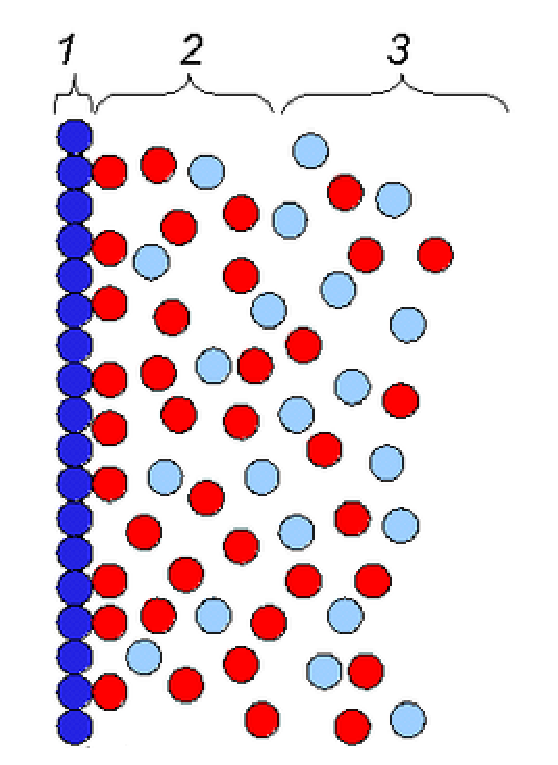
\includegraphics[width=0.25\textwidth]
            {ElectricDoubleLayer.eps}
        \caption{Electrical Double Layer is composed of (1) particle's surface, (2) Debye layer and (3) fluid bulk.
        Zeta potential is defined as the voltage between (1) and (3).}
        \label{fig:EDL}
    \end{center}
\end{framed}
\end{figure}

In case the layer width is much smaller than the particle's size an analytical solution in the Debye-layer can be found \cite{Yariv10a}, and be used as the appropriate boundary condition for the macroscale bulk problem on the particle's surface.

Electrokinetics is described by the following physical phenomena (in dimensionless formulation):
\begin{enumerate}
\item Electrostatic potential - the fluid bulk contains no free charge:
\begin{equation} \label{eq:Laplace}
    \bnabla \cdot (C \bnabla \varPhi) = 0.
\end{equation}
\item Fluid dynamics - Stokes incompressible flow with electrostatic force component:
\begin{equation} \label{eq:Stokes}
\left\{ \begin{array}{l}
\bLaplacian \bV - \bnabla P + \Laplacian \varPhi \bnabla \varPhi = 0 \\
\bnabla \cdot \bV = 0 \end{array} \right.
\end{equation}
\item Ions' diffusion and advection (via fluid's velocity field):
\begin{equation} \label{eq:Nernst}
\Laplacian C - \alpha \bV \cdot \bnabla C = 0
\end{equation}
\end{enumerate}

The boundary conditions correspond to the specific problem at hand and are usually coupled as well as the partial differential equations themselves.

The closed form approximate solution has been developed for spherical particle
and small electric field \cite{Yariv10b} but since the equations are coupled
and non-linear, it is hard to extend the analytic solution to more general
settings.

\section{Research goals}
Our goal is to implement an accurate and fast iterative numerical solver for electrokinetic problems, in cases there are no closed-form solutions known (e.g. asymmetric particles or large electric fields).

The solver will be verified against known closed-form solutions for each of the sub-problems, as well as the full coupled problem, analyzing the discrepancies between the theoretical and numerical results.

Moreover, the convergence rate of the solver will be optimized using numerical acceleration methods to achieve high accuracy in reasonable solver's execution time.

Achieved results will provide a numeric model for interesting small-scale physical phenomena, such as electrophoretic\footnote{Electrophoresis is
the physical phenomenon of particles motion in an ion-containing fluid under the influence of an electric field.} autonomous micro-swimmers \cite{Paxton04, Howse07} by numerically modeling an appropriate particle's configuration.

\section{Achieved results}
The numerical solver is being implemented as a MATLAB package that
provides the needed tools for numerical solution of an electrophoresis problem.

The solver applies iterative relaxations to solve the coupled system, by
iterating the equations and relaxing repeatedly each one of them
for the corresponding variable:
\begin{itemize}
  \item Laplace equation \ref{eq:Laplace} is used to update $\varPhi$.
  \item Stokes equation \ref{eq:Stokes} is used to update $\bV$ and $P$.
  \item Nernst-Planck equation \ref{eq:Nernst} is used to update for $C$.
\end{itemize}
While solving specific equation for a specific variable, all other variables keep their values from previous iteration, resembling ``Gauss-Seidel'' method for non-linear systems.

Problem's configuration is taken from \cite{Yariv10b} and consists of a spherical particle, surrounded by infinite Stokes fluid.
Suppose that the particle is stationary and fluid flows around it, slipping across the boundary layer (due to ``Debye layer'' effects) with a velocity field denoted by $\bV$.

Spherical coordinates $(R,\theta,\phi)$ system is chosen to make the problem axisymmetric around the velocity vector of the fluid, therefore independent of $\phi$.
The electrokinetic problem is written as two-dimensional partial differential equation system for $R \in [1,\infty)$ and $\theta \in [0, \pi]$.
Natural grid choices are a logarithmic grid for $R$ and an uniform grid for $\theta$.

The following linear operators are implemented in spherical coordinates on the grid described above: Scalar Laplacian (for $\varPhi$ and $C$), Vector Laplacian (for $\bV$), Gradient (for $\Phi, C$ and $P$) and Divergence (for $\bV$).

Each differential operator is written in spherical coordinates on the regular $(R, \theta)$ grid and being linear -- is represented as a sparse matrix, making the algebraic manipulations much more straightforward.

The boundary conditions are computed for $\theta = 0$ and $\theta = \pi$ using symmetry considerations. At $R = \infty$, we assume constant fluid velocity and $\bV = \cal{U} \bzhat$, constant electric field $\bnabla \varPhi = -\beta \bzhat$ and constant ionic concentration $C = 1$.
The boundary conditions on $R = 1$ are defined by the boundary layer behavior as described in \cite{Yariv10b}, using Dukhin-�Derjaguin slip formula for $\bV$ and ion-selectivity condition for $\varPhi$ and $C$.

After substitution of boundary conditions, each differential equation is transformed to a sparse linear system of the form $\matr{A}\bx = \vect{b}$.
Due to coupling, it is not necessary to find the exact solution -- so we apply few relaxations on each linear system, using an appropriate preconditioner $\matr{M}_\matr{A}^{-1}$:
\begin{eqnarray} \label{eq:Precond}
  \bx_{n+1} &=& \bx_{n} + \matr{M}_\matr{A}^{-1} \left(\vect{b} - \matr{A}\bx_{n}\right)
\end{eqnarray}

After the solver has converged to a solution for the coupled system, the stress tensor $\mathbb{T}$ on the particle $\cl{S} = \left\{\bx : \|\bx\| = 1\right\}$ is computed  (combining Newtonian and Maxwell stresses) and integrated to yield the total force:
\begin{eqnarray}
  \mathbb{T} &=& - P \mathbb{I} + \bnabla \bV + (\bnabla \bV) ^T  + \bnabla \varPhi \bnabla \varPhi - \frac{\bnabla \varPhi \cdot \bnabla \varPhi}{2} \mathbb{I}, \\
  \vect{F} &=& \int_{\cal{S}} \left(\mathbb{T} \cdot \bnhat \right) ds = \boldsymbol{0}.
\end{eqnarray}
Since the problem is axisymmetric, the force should be aligned with the symmetry axis: $\vect{F} = F \bzhat$.
Moreover, since the particle is stress-free in steady flow, we have $F = 0$ for steady-state velocity $\cal{U}$.

This observation enables us to find the correct $\cal{U}$ for given $\beta$, using one-dimensional root-finding algorithm on $F_\beta(\cal{U})$, as a function of $\cal{U}$.

\section{Algorithms and techniques}

$C$, $\varPhi$ and $P$ are discretized using a central grid whereas staggered grid is used for $\bV$ at the problem domain $\cl{D}$ (see Figure \ref{fig:Grids}).
\begin{figure}[htbp]
\begin{framed}
    \begin{center}
        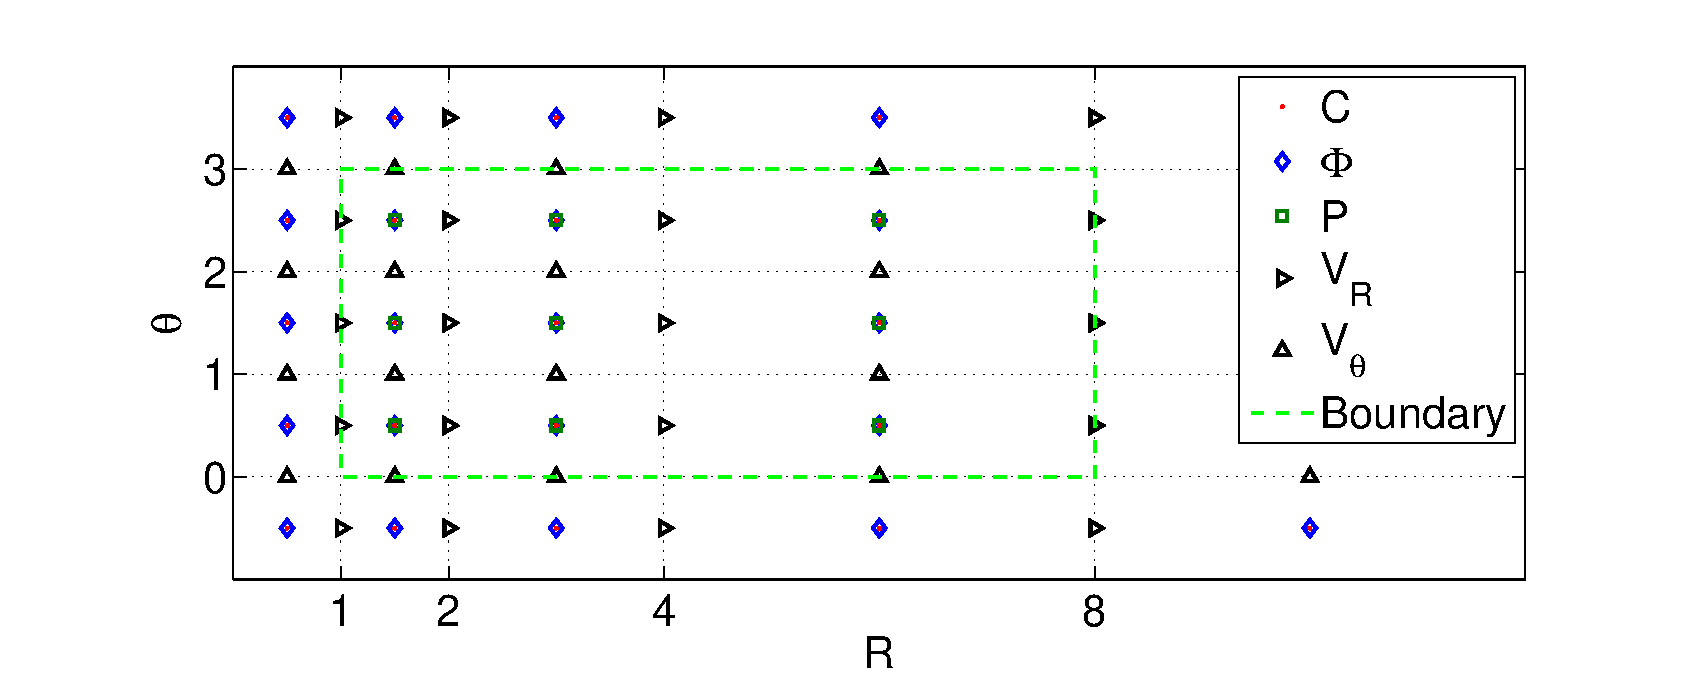
\includegraphics[width=1\textwidth]
            {StaggeredGrid.eps}
        \caption{Grids for $C$, $\varPhi$, $P$ and $\bV$.}
        \label{fig:Grids}
    \end{center}
\end{framed}
\end{figure}


Finite volume method is used to represent the partial differential equations in the form of algebraic system, using
central differences or upwind scheme (for better stability).

``Ghost points'' are used to define Dirichlet and Neumann boundary conditions on
problem domain's boundary $\partial \cl{D}$.

After boundary counditions are eliminated, Jacobi and Red-Black Gauss-Seidel preconditioners are used for equations \ref{eq:Laplace} and \ref{eq:Nernst}, where Vanka-type \cite{Vanka86} preconditioner is used for equation \ref{eq:Stokes}.
The preconditioners are computed as sparse matrices, making the relaxations (at equation \ref{eq:Precond}) much more straightforward.

Vector extrapolation methods \cite{Sidi90} have been implemented and are used to accelerate solver's convergence.
Multigrid solver \cite{Brandt77, Yavneh06} implementation will be a part of the research.

\begin{thebibliography}{}
\bibitem{Yariv10a} E. Yariv,
``An asymptotic derivation of the thin-debye-layer limit for electrokinetic phenomena'',
{\em Chem. Engng Comm. 197, 3�17}, 2010.
\bibitem{Yariv10b} E. Yariv,
``Migration of ion-exchange particles driven by a uniform electric field'',
{\em Journal of Fluid Mechanics, 655 105-121}, 2010.
\bibitem{Rubin01} I. Rubinstein and B. Zaltzman,
``Electro-osmotic slip of the second kind and instability in concentration polarization at electrodialysis membranes'',
{\em Math. Mod. Meth. Appl. Sci. 11 (2), 263�300}, 2001.
\bibitem{Paxton04}
W. Paxton et. al.,
``Catalytic Nanomotors: Autonomous Movement of Striped Nanorods'',
{\em Journal of the American Chemical Society 126 (41), 13424-13431}, 2004.
\bibitem{Howse07}
J. R. Howse et. al.,
``Self-Motile Colloidal Particles: From Directed Propulsion to Random Walk'',
{\em Phys. Rev. Lett., 99, 048102}, 2007.
\bibitem{Vanka86}
S. P. Vanka,
``Block-implicit multigrid solution of Navier-Stokes equations in primitive variables'',
{\em J. Copmput. Phys., 65, 138-158}, 1986.
\bibitem{Sidi90}
A. Sidi, ``Efficient implementation of minimal polynomial and reduced rank extrapolation methods'',
{\em Journal of Computational and Applied Mathematics, Vol. 36, pp. 305-337}, 1991.
\bibitem{Brandt77} Achi Brandt,
``Multi-Level Adaptive Solutions to Boundary-Value Problems'',
{\em Mathematics of Computation, 31: 333�90}, 1977.
\bibitem{Yavneh06} Irad Yavneh.
``Why Multigrid Methods are so Efficient'',
{\em Computing in Science and Engineering, 8(6):12-22}, 2006
\end{thebibliography}

\end{document}
